\section{M\"obius Groups}

\begin{definition}[M\"obius transformation]
A M\"obius transformation (or map) is a function of a complex variable $z$ that can be written in the form 
\begin{align*}
    f(z) = \frac{az + b}{cz + d}
\end{align*} for some $a, b, c, d \in \mathbb{C}$ with $ad - bc \neq 0$.
\end{definition} 

Why $ad - bc \neq 0$?
\begin{align*}
    f(z) - f(w) &= \frac{(ad - bc)(z - w)}{(cz + d) (cw + d)}.
\end{align*} 
So, $ad - bc = 0 \implies f$ is constant (not interesting).
If,  $ad - bc \neq 0 \implies f$ is injective.

When does $f(z) = g(z)$ ($g(z)$ is $f(z)$ with different $a, b, c, d$)?
Suppose $\exists$ at least 3 values of $z$ in $\mathbb{C}$ s.t. 
\begin{align*}
    \frac{az + b}{cz + d} &= \frac{\alpha z + \beta}{\gamma z + \delta} \\
    ad - bc &\neq 0,\ \alpha \delta - \beta \gamma \neq 0.
\end{align*}
Then $\exists \; \lambda \neq 0, \lambda \in \mathbb{C}$ s.t. 
\begin{align*}
    \begin{pmatrix}\alpha & \beta \\\gamma & \delta\end{pmatrix} &= \lambda \begin{pmatrix}a & b \\c & d\end{pmatrix}. 
\end{align*} 
Since, we have 3 distinct values of $z$ for which 
\begin{align*}
    (az + b)(\gamma z + \delta)&= (\alpha z + \beta)(cz + d)
    \intertext{so these quadratics are identical}
    \implies \alpha \gamma &= \alpha c,\ b \delta = \beta d \\
    a \delta + \beta \delta &= \alpha d + \beta c \\
    \text{Let } \mu &= a \delta - \beta c = \alpha d - b \gamma \\
    (\text{so } \mu^2 &= (ad - bc)(\alpha \delta - \beta \gamma) \neq 0). \\
    \text{Then } \begin{pmatrix}d & -b \\-c & a\end{pmatrix} \begin{pmatrix}\alpha & \beta \\\gamma & \delta\end{pmatrix} &= \begin{pmatrix}\mu & 0 \\0 & \mu\end{pmatrix} \\
    \implies \begin{pmatrix}\alpha & \beta \\\gamma & \delta\end{pmatrix} &= \frac{\mu}{ad - bc} \begin{pmatrix}a & b \\c & d\end{pmatrix}.
\end{align*} 

Problem: $f$ is not defined at $z = - \frac{d}{c}$.
We would like $f(-\frac{d}{c}) = \infty$.
We consider $f$ defined on $\mathbb{C} \cup \{ \infty \} = \mathbb{C}_\infty$ the extended complex plane.
So if $f(z) = \frac{az + b}{cz + d}$, domain is now $\mathbb{C}_\infty$.
If $c \neq 0;\ f(\infty) = \frac{a}{c};\ f(-\frac{d}{c}) = \infty$ else $c = 0;\ f(\infty) = \infty$.

\begin{figure}
    \centering
    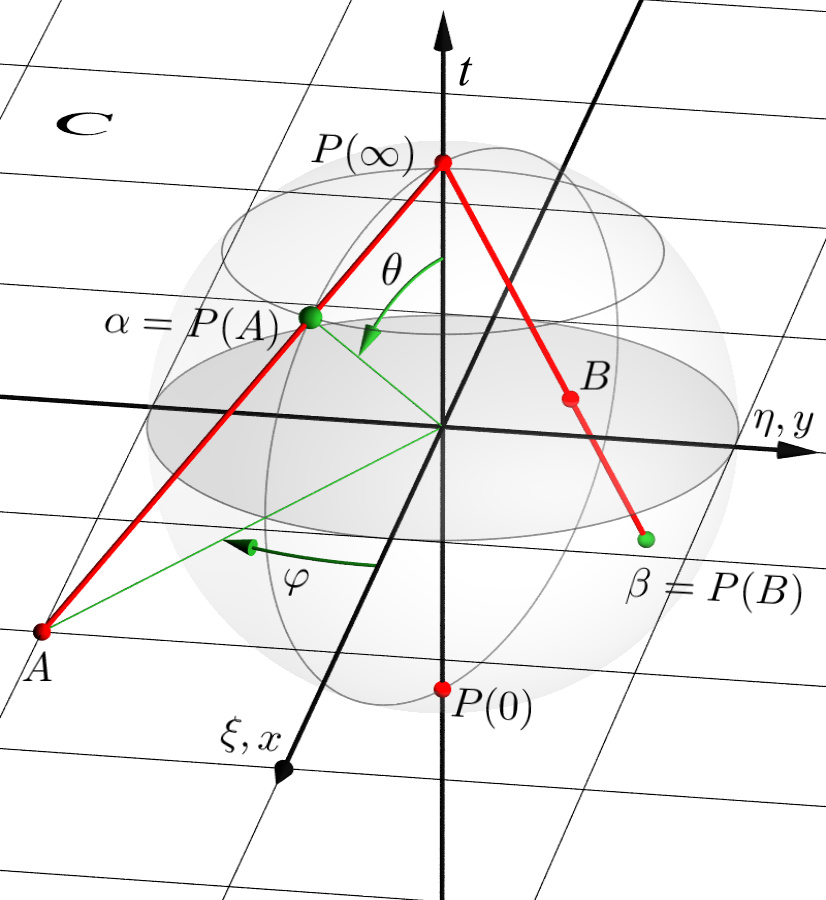
\includegraphics[height=5cm]{07-RiemannSphere}
    \caption{Stereographic projection of a complex number $A$ onto a point $\alpha$ of the Riemann sphere}
\end{figure} 

\begin{theorem}\label{thm:14}
    The set $\mathcal{M}$ of all M\"obius maps on $\mathbb{C}_\infty$ is a group under composition.
    It is a subgroup of $\operatorname{Sym}(\mathbb{C}_\infty)$.
\end{theorem} 

\begin{proof}
    \begin{itemize}
        \item Composition of maps is associative.
        \item $I(z) = z \in \mathcal{M}$ ($a = d = 1, b = c = 0$)
        \item closure:
        \begin{align*}
            \text{Let } f(z) &= \frac{az + b}{cz + d},\ g(z) = \frac{\alpha z + \beta}{\gamma z + \delta} \\
            \text{Suppose } c &\neq 0,\ \delta \neq 0 \\
            \text{First suppose } z &\in \mathbb{C} \setminus \{ - \delta / \gamma \} \\
            \text{Then } f(g(z)) &=  \frac{a \left( \frac{\alpha z + \beta}{\gamma z + \delta} \right) + b}{c \left( \frac{\alpha z + \beta}{\gamma z + \delta} \right) + d} \\
            &= \frac{(a \alpha + b \gamma) z + (a \beta + b \delta)}{(c \alpha + d \gamma)z + (c \beta + \delta d)} \\
            &\in \mathcal{M}
            \intertext{since $(a \alpha + b \gamma)(c \beta + \delta d) - (a \beta + b \delta)(c \alpha + d \gamma) = (ad - bc)(\alpha \delta - \beta \gamma) \neq 0$}
            \text{Also, } f\left(g\left(-\frac{\delta}{\gamma}\right)\right) &= f(\infty) = \frac{a}{c} \\
            \text{and } \frac{(a \alpha + b \gamma) \left(-\frac{\delta}{\gamma}\right) + (a \beta + b \delta)}{(c \alpha + d \gamma)\left(-\frac{\delta}{\gamma}\right) + (c \beta + \delta d)} &= \frac{a \alpha \left(-\frac{\delta}{\gamma}\right) + a \beta}{c \alpha \left(-\frac{\delta}{\gamma}\right) + c \beta} \\
            &= \frac{a}{c} \ \checkmark \\
            \text{Need to check } c &= 0
        \end{align*} 
        \item Inverses: 
        \begin{align*}
            f(z) &= \frac{az + b}{cz + d},\ ad - bc \neq 0 \\
            \text{Let } f^*(z) &= \frac{dz - b}{-cz + a} \\
            \text{Then } f(f^*(z)) &= z = f^*(f(z)) \text{ for } z \neq -\frac{d}{c}, -\frac{a}{c}, \infty 
            \intertext{These cases are ok.}
            \text{If } c &= 0 \\
            f(f^*(\infty)) &= f(\infty) = \infty = f^*(f(\infty)).
        \end{align*}
    \end{itemize} 
\end{proof} 

\begin{theorem}\label{thm:15}
    $\operatorname{GL}_2(\mathbb{C}) / Z \cong \mathcal{M}$ where $Z = \left\{ \begin{pmatrix}\lambda & 0 \\0 & \lambda\end{pmatrix} : \lambda \in \mathbb{C} \setminus \{0\} \right\}$ ($Z$ is the centre of $\operatorname{GL}_2(\mathbb{C})$).
\end{theorem} 

\begin{proof}
    We construct a surjective homomorphism from $\operatorname{GL}_2(\mathbb{C})$ onto $\mathcal{M}$ with kernel $Z$.
    \begin{align*}
        \text{Let } \Phi : \operatorname{GL}_2(\mathbb{C}) &\to \mathcal{M} \\
        \begin{pmatrix}a & b \\c & d\end{pmatrix} &\mapsto f(z) = \frac{az + b}{cz + d}
        \intertext{Note $\Phi$ is a homomorphism}
        f(z) &= \frac{az + b}{cz + d},\ g(z) = \frac{\alpha z + \beta}{\gamma z + \delta} \\
        \Phi \left( \begin{pmatrix}a & b \\c & d\end{pmatrix} \right) &\Phi \left( \begin{pmatrix}\alpha & \beta \\\gamma & \delta\end{pmatrix} \right) (z) = f \circ g(z) \\
        &= \frac{(a \alpha + b \gamma) z + (a \beta + b \delta)}{(c \alpha + d \gamma)z + (c \beta + \delta d)} \text{ from proof of \Cref{thm:14}} \\
        &= \Phi \left( \begin{pmatrix}a & b \\c & d\end{pmatrix} \begin{pmatrix}\alpha & \beta \\\gamma & \delta\end{pmatrix} \right) (z).
    \end{align*} 
    Clearly $\Phi$ is surjective.
    \begin{align*}
        \begin{pmatrix}a & b \\c & d\end{pmatrix} &\in \ker \Phi \\
        \iff \frac{az + b}{cz + d} &= z \; \forall \; z \in C_\infty \\
        \text{Let } z &= \infty \implies c = 0 \\
        z &= 0 \implies b = 0 \\
        z &= 1 \implies a = d \\
        \implies \ker \Phi &= Z
    \end{align*} 
    Finally apply \nameref{thm:six}.
\end{proof} 

\begin{corollary} \label{cor:7} ~\vspace*{-1.5\baselineskip}
    \begin{align*}
        \frac{\operatorname{SL}_2(\mathbb{C})}{\{ \pm I \}} &= \mathcal{M}.
    \end{align*} 
\end{corollary} 

\begin{proof}
    Restrict $\phi$ to $\operatorname{SL}_2(\mathbb{C})$
    \begin{align*}
        \Phi : \operatorname{SL}_2(\mathbb{C}) &\to \mathcal{M} \\
        \begin{pmatrix}a & b \\c & d\end{pmatrix} &\mapsto \frac{az + b}{cz + d}
    \intertext{We require $\Phi$ to be surjective:}
        f(z) &= \frac{az + b}{cz + d} \\
        &= \frac{ \frac{a}{\sqrt{ad - bc}} z + \frac{b}{\sqrt{ad - bc}} }{ \frac{c}{\sqrt{ad - bc}} z + \frac{d}{\sqrt{ad - bc}} }.
    \end{align*} 
    And $\ker \Phi = \{ \pm I \}$.
\end{proof} 

\begin{proposition} \label{prp:13}
    Every M\"obius map can be written as a composition of maps of the following forms:
    \begin{enumerate}
        \item $z \mapsto az$, $a \neq 0$; represents a dilation or a rotation \label{itm:1-1}
        \item $z \mapsto z + b$; a translation \label{itm:1-2}
        \item $z \mapsto \frac{1}{z}$; inversion. \label{itm:1-3}
    \end{enumerate} 
\end{proposition} 

\begin{proof}
    Let $f(z) = \frac{az + b}{cz + d}$. \\
    \begin{align*}
        \text{If } c&= 0;\ z \mapsto \underbrace{\left(\frac{a}{d} \right) z}_{f_1,\ \Cref{itm:1-1}} \mapsto \underbrace{\left( \frac{a}{d} \right) z + \frac{b}{d}}_{f_2,\ \Cref{itm:1-2}} \\
        f &= f_2 \circ f_1 \\
        \text{If } c &\neq 0 \\
        f(z) &= \frac{az + b}{cz + d} = \frac{\left( \frac{a}{c} \right) z + \left( \frac{b}{c} \right)}{z + \left( \frac{d}{c} \right)} \\
        &= \left( \frac{a}{c} \right) + \frac{\frac{-ad + bc}{c^2}}{z + \frac{d}{c}} \\
        &= A + \frac{B}{z + \frac{d}{c}},\ B \neq 0 \\
        z &\underset{f_1,\ \Cref{itm:1-2}}{\mapsto} z + \frac{d}{c} \\
        &\underset{f_2,\ \Cref{itm:1-3}}{\mapsto} \frac{1}{z + \frac{d}{c}} \\
        &\underset{f_3,\ \Cref{itm:1-1}}{\mapsto} \frac{B}{z + \frac{d}{c}} \\
        &\underset{f_4,\ \Cref{itm:1-2}}{\mapsto} A + \frac{B}{z + \frac{d}{c}} \\
        f &= f_4 \circ f_3 \circ f_2 \circ f_1
    \end{align*} 
\end{proof} 

\begin{definition}[Triply transitive action] \label{def:22}
    A group $G$ acts \emph{triply transitively} on a set $X$ if given $x_1, x_2, x_3 \in X$ all distinct and $y_1, y_2, y_3 \in X$ all distinct there exists $g \in G$ such that $g(x_i) = y_i,\ i = 1, 2, 3$. \\
    A group $G$ acts \emph{sharply triply transitively} if such a $g$ is unique.
\end{definition} 

\begin{theorem} \label{thm:16}
    The action of $\mathcal{M}$ on $\mathbb{C}_\infty$ is sharply triply transitive.
\end{theorem} 

\begin{proof}
    Label first triple $\{z_0, z_1, z_\infty\}$ and second triple $\{w_0, w_1, w_\infty\}$.
    We construct $g \in \mathcal{M}$ s.t.
    \begin{align*}
        g : z_0 &\mapsto 0 \\
        z_1 &\mapsto 1 \\
        z_\infty &\mapsto \infty.
    \intertext{First suppose $z_0, z_1, z_\infty \neq \infty$}
        g(z) &= \frac{(z - z_0) (z_1 - z_\infty)}{(z - z_\infty) (z_1 - z_0)} \\
        \text{Check: } ``ad - bc" &= (z_0 - z_\infty)(z_1 - z_\infty)(z_1 - z_0) \neq 0.
    \intertext{If $z_\infty = \infty$}
        g(z) &= \frac{(z - z_0)}{(z_1 - z_0)}
    \intertext{If $z_1 = \infty$}
        g(z) &= \frac{(z - z_0)}{(z - z_\infty)}
    \intertext{If $z_0 = \infty$}
        g(z) &= \frac{(z_1 - z_\infty)}{(z - z_\infty)}
    \intertext{Similarly find $h$ s.t.}
    g : w_0 &\mapsto 0 \\
        w_1 &\mapsto 1 \\
        w_\infty &\mapsto \infty. \\
    \text{Then } f = h^{-1} g : z_i &\to w_i
    \end{align*} 
    Now to prove uniqueness.
    \begin{align*}
        \text{Suppose } f' : z_i &\mapsto w_i \\
        \text{Then } f^{-1} \circ f' : z_i &\mapsto z_i
        \intertext{Let $g$ be as above}
        g f^{-1} f' g^{-1} : 0 &\mapsto 0 \implies b = 0 \\
        : 1 &\mapsto 1 \implies a = d \\
        : \infty &\mapsto \infty \implies c = 0 \\
        \implies g f^{-1} f' g^{-1} &= \text{id} \\
        \implies f^{-1} f' &= \text{id} \\
        \implies f &= f'.
    \end{align*} 
    So, the image of just three points determines the map
\end{proof} 

\subsection{Conjugacy classes in \texorpdfstring{$\mathcal{M}$}{ℳ}}
Recall $\Phi : \operatorname{GL}_2(\mathbb{C}) \twoheadrightarrow \mathcal{M}$ from proof of \Cref{thm:15} ($\twoheadrightarrow$ means its a surjective homomorphism).
Suppose $A, B$ are conjugate in $\operatorname{GL}_2(\mathbb{C})$, i.e. $\exists \; P \in \operatorname{GL}_2(\mathbb{C})$ s.t. $PAP^{-1} = B$ then
\begin{align*}
    \Phi(P) \Phi(A) \Phi(P)^{-1} &= \Phi(PAP^{-1}) \\
    &= \Phi(B) \in \mathcal{M}
\end{align*} 
i.e. $\Phi(A)$ and $\Phi(B)$ are conjugate in $\mathcal{M}$.

Use knowledge of conjugacy classes in $\operatorname{GL}_2(\mathbb{C})$.

\begin{theorem} \label{thm:17}
    Any non-identity M\"obius map is conjugate to $f(z) = \nu z$ for some $\nu \neq 0, 1$ or to $f(z) = z + 1$.
\end{theorem} 

\begin{proof} ~
    \begin{enumerate}
        \item
        \begin{align*}
            \begin{pmatrix}\lambda & 0 \\0 & \mu\end{pmatrix} \text{ where } \lambda &\neq \mu,\ \lambda \neq 0 \neq \mu. \\
            \Phi \left( \begin{pmatrix}\lambda & 0 \\0 & \mu\end{pmatrix} \right) &= f,\ f(z) = \frac{\lambda}{\mu} z = \nu z,\ \nu \neq 0, 1.
        \end{align*}
        \item
        \begin{align*}
            \begin{pmatrix}\lambda & 0 \\0 & \mu\end{pmatrix} \text{ where } \lambda &\neq 0 \\
            \Phi \left( \begin{pmatrix}\lambda & 0 \\0 & \lambda \end{pmatrix} \right) &= \text{id}.
        \end{align*}
        \mathitem \begin{align*}
            \begin{pmatrix}\lambda & 1 \\0 & \lambda\end{pmatrix} \text{ where } \lambda &\neq 0 \\
            \Phi \left( \begin{pmatrix}\lambda & 1 \\0 & \lambda \end{pmatrix} \right) &= f,\ f(z) = \frac{\lambda z + 1}{\lambda} = z + \frac{1}{\lambda} \\
            \text{i.e. } f &= \Phi \left( \begin{pmatrix}1 & \frac{1}{\lambda} \\0 & 1\end{pmatrix} \right). \\
            \text{And } \begin{pmatrix}1 & \frac{1}{\lambda} \\0 & 1\end{pmatrix} &\text{ is conjugate to } \begin{pmatrix}1 & 1 \\0 & 1\end{pmatrix} \\ 
            \text{ via } \begin{pmatrix}\lambda & 0 \\ 0 & 1 \end{pmatrix}  \begin{pmatrix}1 & \frac{1}{\lambda} \\0 & 1\end{pmatrix} \begin{pmatrix}\frac{1}{\lambda} & 0 \\ 0 & 1 \end{pmatrix} &= \begin{pmatrix}1 & 1 \\0 & 1\end{pmatrix}.
        \end{align*}
        So $f$ is conjugate to $g$ where $g(z) = z + 1$.
    \end{enumerate} 
\end{proof} 

\begin{corollary} \label{cor:8}
    A non-identity M\"obius map has either 
    \begin{enumerate}
        \item 2 fixed points or
        \item 1 fixed point.
    \end{enumerate} 
\end{corollary} 

\begin{proof}
    Suppose $g f g^{-1} = h$.
    Then $\alpha$ is a fixed point of $f$ (i.e. $f(\alpha) = \alpha$) $\iff$ $g(\alpha)$ is a fixed point of $h$ (i.e. $h(g(\alpha)) = g(\alpha)$).\footnote{$f(\alpha) = \alpha \iff gf(\alpha) = g(\alpha) \iff h(g(\alpha)) = gfg^{-1}(g(\alpha)) = g(\alpha)$ or $g f = h g \implies h(g(\alpha)) = g(\alpha)$ if $f(\alpha) = \alpha$ and conversely $g(f(\alpha)) = h(g(\alpha)) \implies g(f(\alpha)) = g(\alpha)$.} \\
    So number of fixed points of $f = $ number of fixed points of $h$ as $g$ is a bijection.
    By \Cref{thm:17} either, $f$ conjugate to $z \mapsto \nu z$ which has two fixed points: $0, \infty$; or $f$ conjugate to $z \mapsto z + 1$ which has one fixed point: $\infty$.
\end{proof} 

\subsection{Circles in $\mathbb{C}_\infty$}

A Euclidean circle is the set of points in $\mathbb{C}$ given by some equation $|z - z_0| = r,\ r > 0$.
A Euclidean line is the set of points in $\mathbb{C}$ given by some equation $|z - a| = |z - b|,\ a \neq b$.

\begin{definition}[Circle in $\mathbb{C}_\infty$]
    A \emph{circle in $\mathbb{C}_\infty$} is either a Euclidean circle or a set $L \cup \{\infty\}$ where $L$ is a Euclidean line.
    Its general equation is of the form 
    \begin{align}
        Az\bar z + \bar Bz + B\bar z + C = 0, \label{eq:circle}
    \end{align} 
    where $A, C \in \mathbb{R}$ and $|B|^2 > AC$.
\end{definition}

Where $z = \infty$ is a solution iff $A = 0$. \\
$A = 0$: line \\
$C = 0$: goes through the origin.

There is a unique circle passing through any 3 distinct points in $\mathbb{C}_\infty$.

\begin{theorem} \label{thm:18}
    Let $f \in \mathcal{M}$ and $C$ a circle in $\mathbb{C}_\infty$, then $f(C)$ is a circle in $C_\infty$.
\end{theorem} 

\begin{proof}
    By \Cref{prp:13}, just need to consider 
    $f(z) = az,\ z + b \text{ or } \frac{1}{z}.$
    Let $S_{A, B, C}$ be the circle defined by \Cref{eq:circle}.
    \begin{align*}
        f(z) &= az : S_{A, B, C} \mapsto S_{A / a \bar{a}, B / \bar{a}, C} \\
        f(z) &= z + b: S_{A, B, C} \mapsto S_{A, B - Ab, C + A b \bar{b} - \bar{B}b - B \bar{b}} \\
        f(z) &= \frac{1}{z} = w: S_{A, B, C} \mapsto A + B w + \bar{B} \bar{w} + C w \bar{w} = 0 = S_{C, \bar{B}, A}.
    \end{align*} 
\end{proof} 

\begin{example}
    Consider the image of $\mathbb{R} \cup \{\infty\}$ (a circle in $\mathbb{C}_\infty$) under 
    \begin{align*}
        f(z) &= \frac{z - i}{z + i}.
    \end{align*}
    It is thus a circle in $\mathbb{C}_\infty$ containing $f(0) = -1, f(\infty) = 1, f(1) = -i$ so $f(\mathbb{R} \cup \{\infty\}) = $ unit circle. 
    Furthermore, complimentary components are mapped to complimentary components.
    {\centering 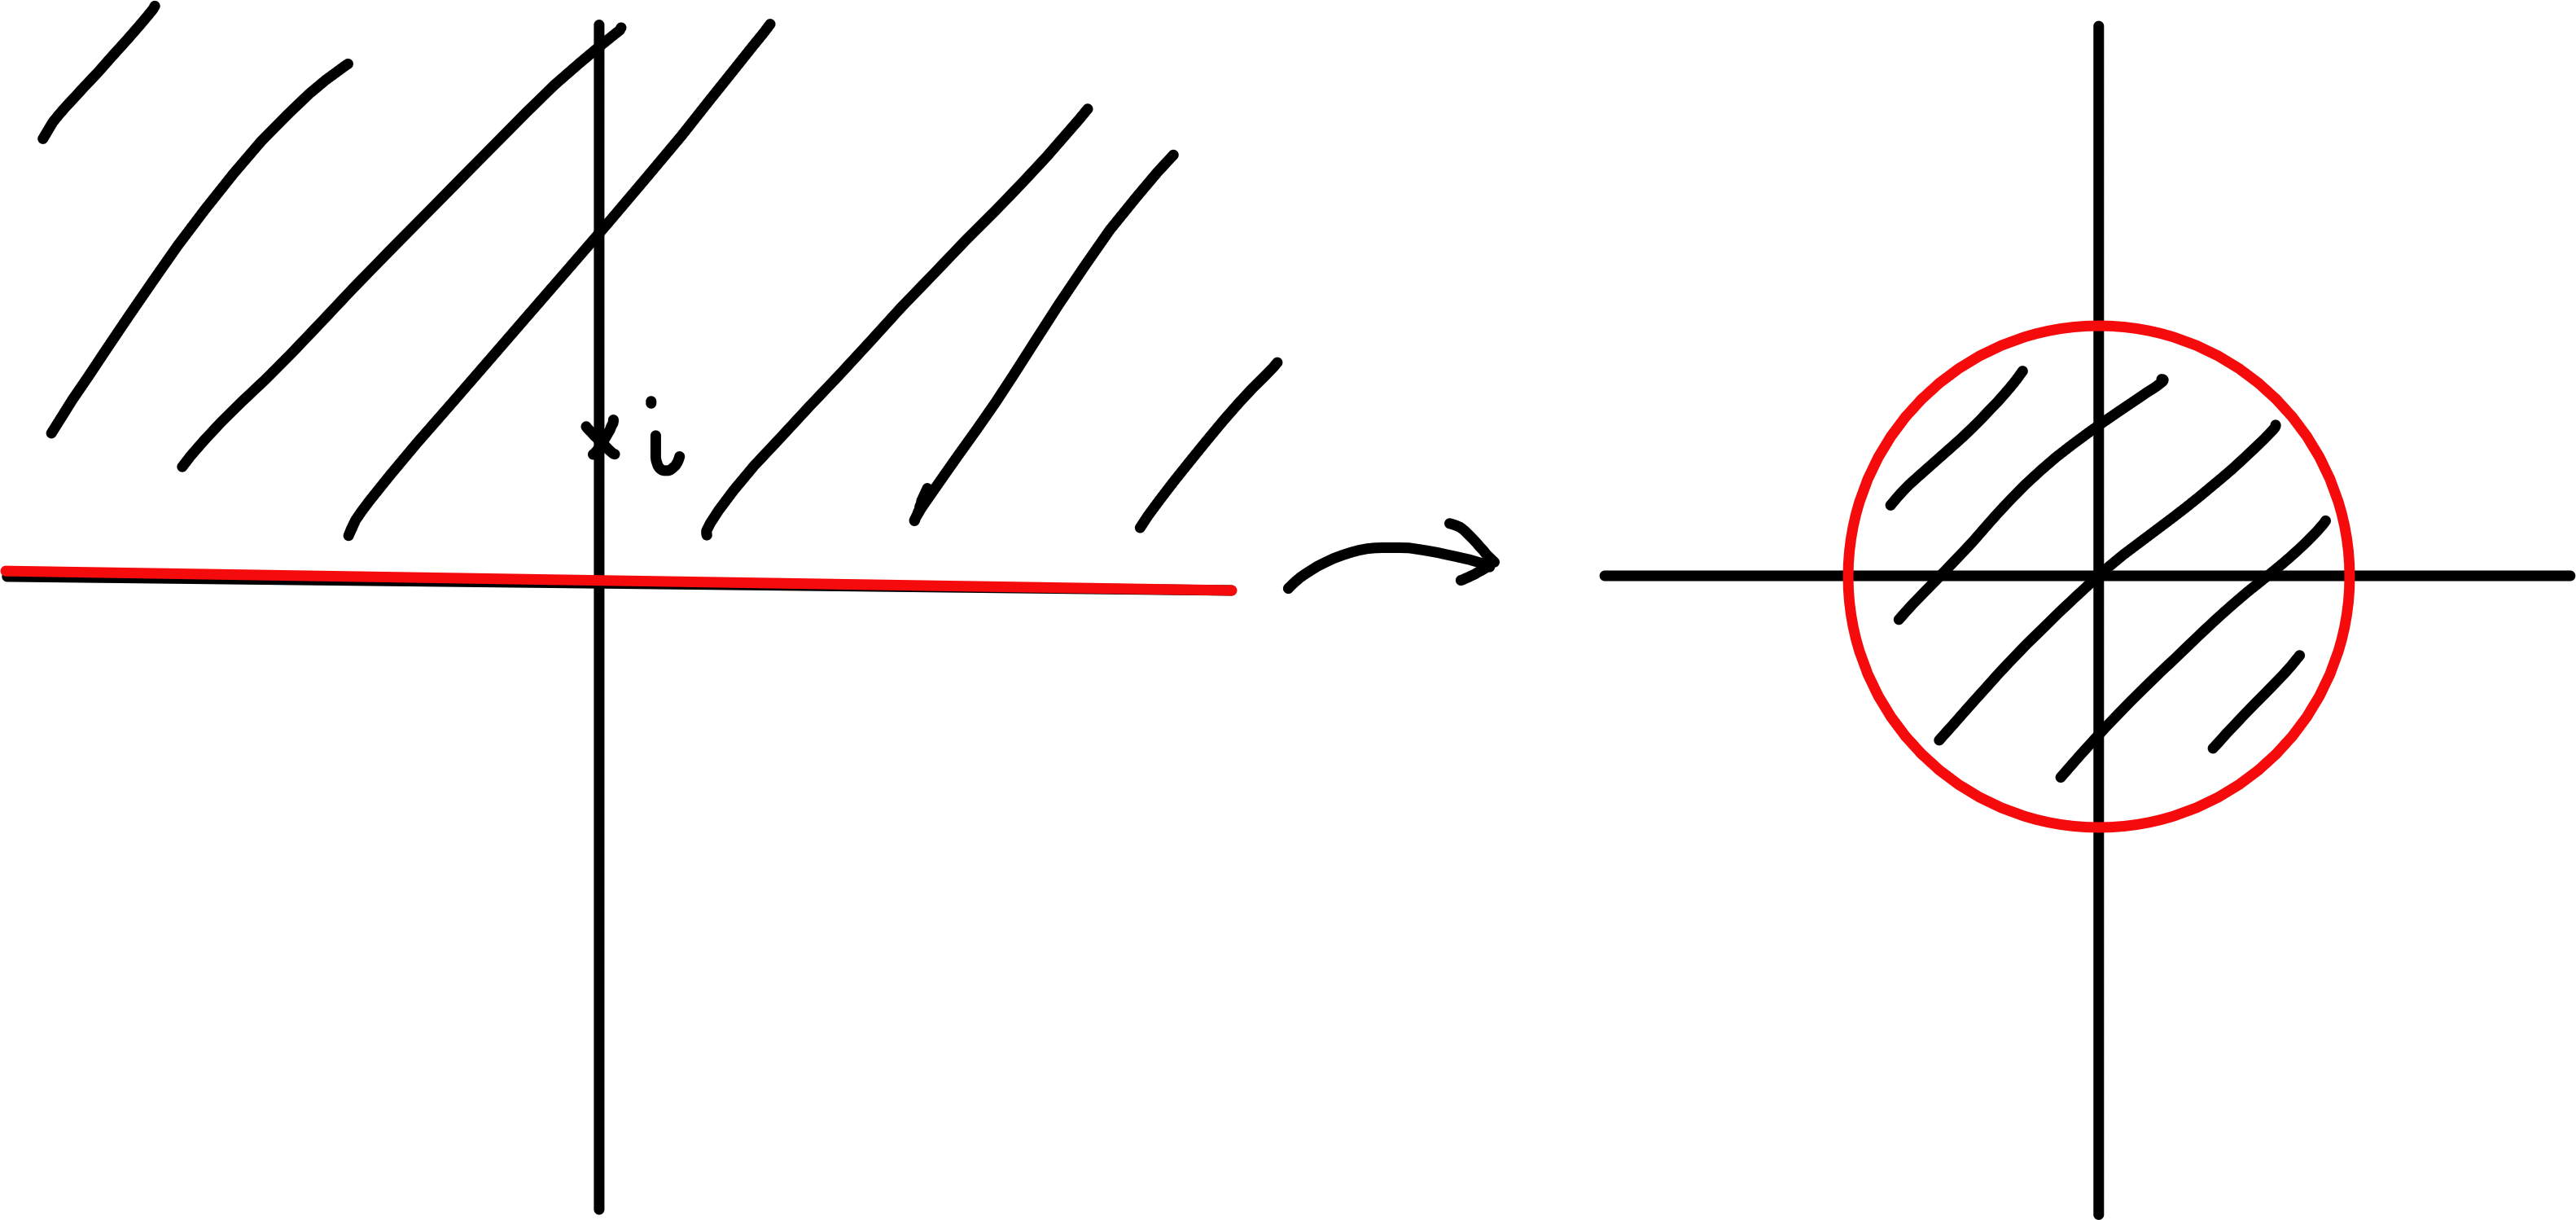
\includegraphics[height=5cm]{08-complimentary}}
\end{example} 

\subsection{Cross-Ratios}

\begin{definition} \label{def:23}
    The cross-ratio of distinct points $z_1, z_2, z_3, z_4 \in \mathbb{C}$.
    \begin{align*}
        [z_1, z_2, z_3, z_4] &= \frac{(z_1 - z_3)(z_2 - z_4)}{(z_1 - z_2)(z_3 - z_4)} \\
        [\infty, z_2, z_3, z_4] &= \frac{(z_2 - z_4)}{(z_3 - z_4)} \\
        [z_1, \infty, z_3, z_4] &= -\frac{(z_1 - z_3)}{(z_3 - z_4)} \\
        [z_1, z_2, \infty, z_4] &= -\frac{(z_2 - z_4)}{(z_1 - z_2)} \\
        [z_1, z_2, z_3, \infty] &= \frac{(z_1 - z_3)}{(z_1 - z_2)} \\
    \end{align*} 
\end{definition} 

Note $[0, 1, w, \infty] = \frac{-w}{-1} = w$

\emph{Warning}: different authors use different permutations of $1, 2, 3, 4$ in the definition.

\begin{theorem} \label{thm:19}
    Given $z_1, z_2, z_3, z_4 \in \mathbb{C}_\infty$ distinct $w_1, w_2, w_3, w_4 \in \mathbb{C}_\infty$ distinct then $\exists \; f \in \mathcal{M}$ s.t. $f(z_i) = w_i \iff [z_1, z_2, z_3, z_4] = [w_1, w_2, w_3, w_4]$.
    In particular, M\"obius maps preserve cross-ratios $[z_1, z_2, z_3, z_4] = [f(z_1), f(z_2), f(z_3), f(z_4)]$
\end{theorem} 

\begin{proof} ~
    ($\implies$): Suppose $f(z_j) = w_j$ and $z_i, w_i \neq \infty \quad \forall \; i$ and $f(z) = \frac{az + b}{cz + d}$, then $cz_j + d \neq 0 \quad \forall \; j$.
    \begin{align*}
        \text{So, } w_j - w_k &= f(z_j) - f(z_k) \\
        &= \frac{(ad - bc) (z_j - z_k)}{(c z_j + d) (c z_k + d)} \\
        \implies [z_1, z_2, z_3, z_4] &= [w_1, w_2, w_3, w_4] \\
        &=  [f(z_1), f(z_2), f(z_3), f(z_4)]
    \end{align*} 
    Need to check other cases; $z_1 = \infty, w_1 = f(\infty) = \frac{a}{c}$ etc.

    ($\Longleftarrow$): Suppose $[z_1, z_2, z_3, z_4] = [w_1, w_2, w_3, w_4]$.
    Let $g \in \mathcal{M}$ s.t. $g(z_1) = 0, g(z_2) = 1, g(z_4) = \infty$ as triple transitive.
    Let $h \in \mathcal{M}$ s.t. $h(w_1) = 0, h(w_2) = 1, h(w_4) = \infty$.
    \begin{align*}
        g(z_3) &= [0, 1, g(z_3), \infty] \\
        &= [g(z_1), g(z_2), g(z_3), g(z_4)] \\
        &= [z_1, z_2, z_3, z_4] \text{ by above} \\
        &= [w_1, w_2, w_3, w_4] \\
        &= [h(w_1), h(w_2), h(w_3), h(w_4)] \\
        &= [0, 1, h(w_3), \infty] \\
        &= h(w_3).
    \end{align*} 
    So $h^{-1}g$ is required map. 
\end{proof} 

So $[z_1, z_2, z_3, z_4] = f(z_3)$ where $f$ is the unique M\"obius map that sends $z_1 \mapsto 0,\ z_2 \mapsto 1,\ z_4 \mapsto \infty$.

\begin{corollary} \label{cor:9}
    $z_1, z_2, z_3, z_4$ lie in some circle in $\mathbb{C}_\infty \iff [z_1, z_2, z_3, z_4] \in \mathbb{R}$.
\end{corollary} 

\begin{proof}
    Let $C$ be a circle through $z_1, z_2, z_4$. \\
    Let $g : C \to \mathbb{R} \cup \{\infty\}$ s.t. $g(z_1) = 0,\ g(z_2) = 1,\ g(z_4) = \infty$.
    \begin{align*}
        g(z_3) &= [0, 1, g(z_3), \infty] \\
        &= [g(z_1), g(z_2), g(z_3), g(z_4)] \\
        &= [z_1, z_2, z_3, z_4] \text{ by \Cref{thm:19}} \\
        \text{So, } [z_1, z_2, z_3, z_4] \in \mathbb{R} &\iff g(z_3) \in \mathbb{R} \\
        &\iff z_3 \in C.
    \end{align*} 
\end{proof} 